\section{Effect of Height}

As can be seen in (\ref{eq:camera_position_body}), the effect the pitch and roll has on the camera position increases proportionally with the altitude of the aircraft. In Figure \ref{fig:opt_height} a $45\degree$ curved turn has been optimized with the aircraft flying at different altitudes, namely $100$m, $200$m and $300$m. While the altitude do not affect the path the MPC chooses to fly the aircraft, the effect is easily visible in the camera position shown in Figure \ref{fig:opt_height_camera}. When flying at an altitude of $100$m the camera position takes the inner turn, while for $300$m it greatly widens the turn. The optimization fails to return a stable result at an altitude of $400$m.

\begin{figure}
	\makebox[\textwidth][c]{
	\subfloat[UAV position]{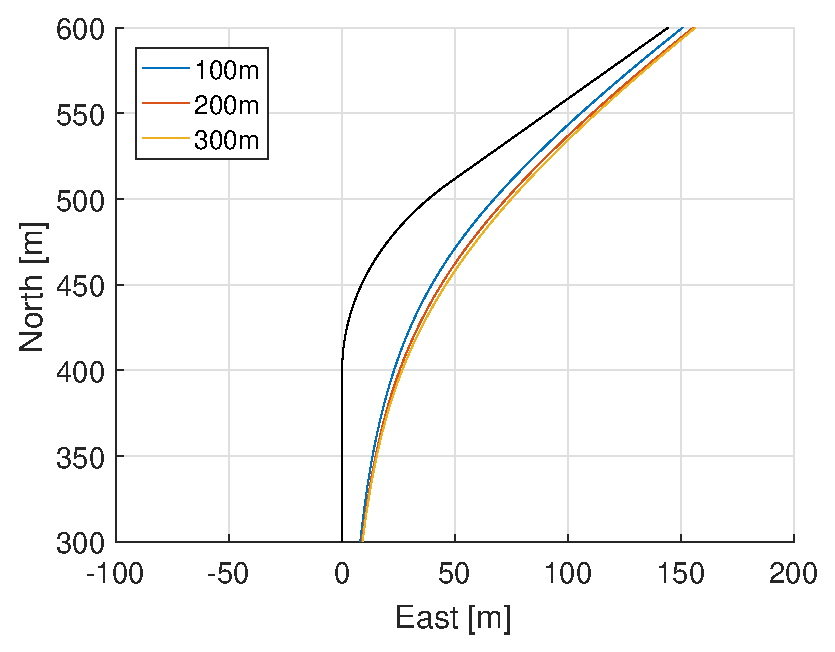
\includegraphics[width=0.5\textwidth, keepaspectratio=true]{../../results/opt/height/fig_cur/uav_pos.eps}}
	\qquad
	\subfloat[Camera position]{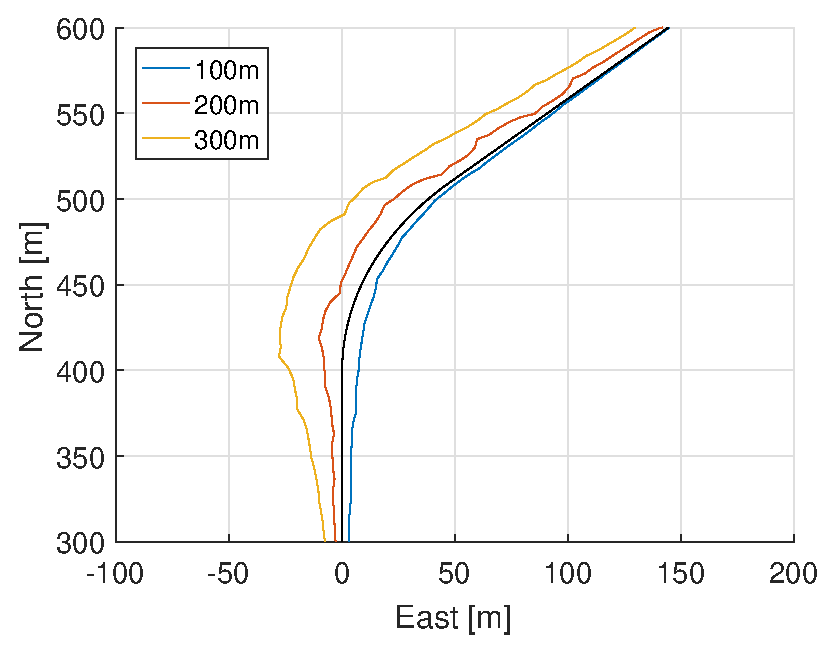
\includegraphics[width=0.5\textwidth, keepaspectratio=true]{../../results/opt/height/fig_cur/camera_pos.eps}
	\label{fig:opt_height_camera}}}
	\caption{The UAV and camera position when tracking a $45\degree$ turn with $200$m radius at different altitudes.}
	\label{fig:opt_height}
\end{figure}